\section{Results}

\subsection{Experimental Setup}
SpiderMark is evaluated on a diverse suite of image perturbations to assess watermark detectability and robustness under real-world transformations. 
Experiments are conducted using a Stable Diffusion v2.1 backbone, where the watermark is injected into the initial noise tensor \(x_T\). 
The verification model is trained to classify between watermarked and non-watermarked images in the frequency domain, while a PSNR-based detector with a fixed sigmoid threshold of \(-4\) serves as the baseline.

Nine types of image transformations are applied:  
(1) \textit{clean}, (2) \textit{jpeg\_strong}, (3) \textit{msg\_app\_combo}, (4) \textit{down\_up}, (5) \textit{blur}, (6) \textit{random\_crop}, (7) \textit{occlusion}, (8) \textit{geom\_warp}, and (9) \textit{train\_aug\_mix}.  
These augmentations simulate practical degradations such as compression, scaling, occlusion, and geometric distortion commonly seen in content sharing platforms.


\paragraph{Verifier Training Details.}
We sample prompts from the public \texttt{Gustavosta/Stable-Diffusion-Prompts} collection and generate a balanced dataset of 500 watermarked and 500 non-watermarked images using Stable Diffusion v2.1.
All images are converted to grayscale, transformed using a 2D FFT, and the magnitude spectrum is provided to a ResNet-18 verifier pretrained on ImageNet.
The model is fine-tuned using binary cross-entropy loss.

% %%% TODO: 5x5 matrix - find 5 examples and show the five algorithms
% \begin{figure*}[t]
%     \centering

%     % ---- Row 1 ----
%     \begin{subfigure}[b]{0.31\linewidth}
%         \centering
%         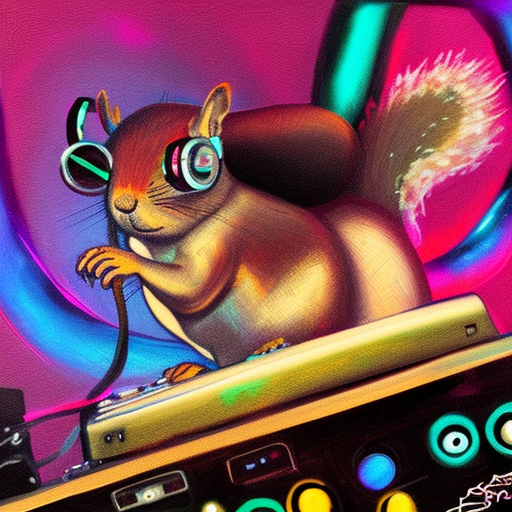
\includegraphics[width=\linewidth]{clean_image.png}
%         \caption{Clean Image}
%     \end{subfigure}
%     \hfill
%     \begin{subfigure}[b]{0.31\linewidth}
%         \centering
%         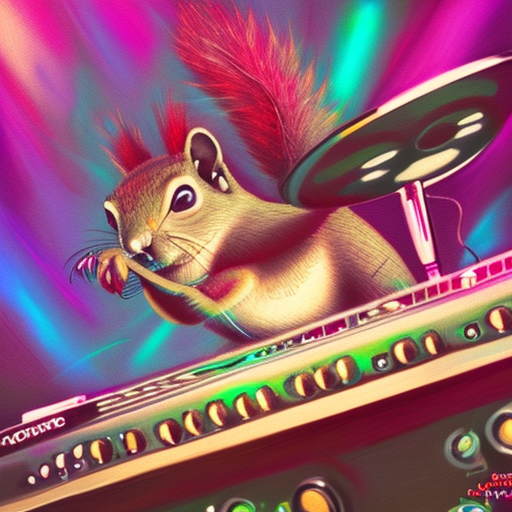
\includegraphics[width=\linewidth]{spidernet_watermarked.png}
%         \caption{SpiderMark Watermark}
%     \end{subfigure}
%     \hfill
%     \begin{subfigure}[b]{0.31\linewidth}
%         \centering
%         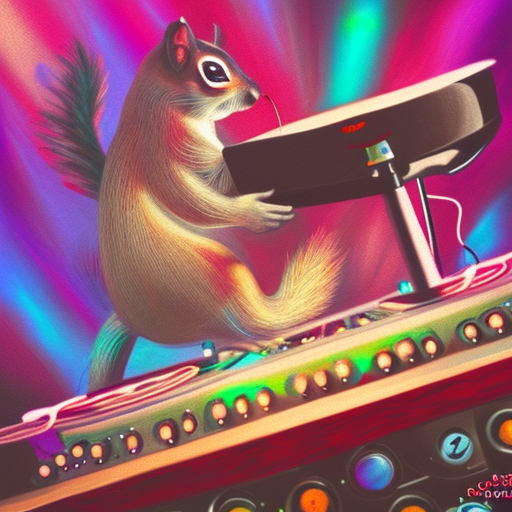
\includegraphics[width=\linewidth]{ring_watermarked.png}
%         \caption{Ring Watermarked}
%     \end{subfigure}

%     \vspace{6mm}

%     % ---- Row 2 ----
%     \begin{subfigure}[b]{0.49\linewidth}
%         \centering
%         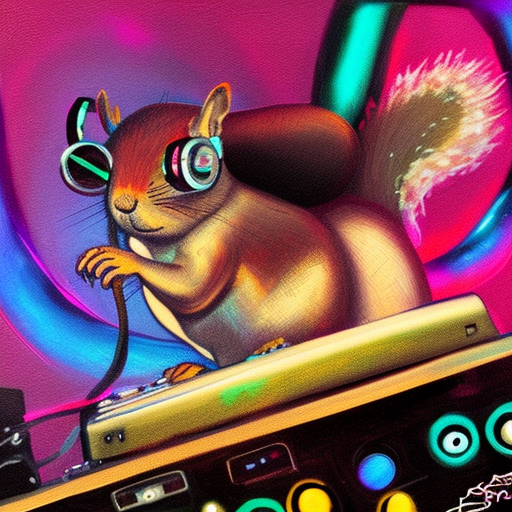
\includegraphics[width=0.62\linewidth]{dft_single_str10.PNG}
%         \caption{DFT-Single Watermark}
%     \end{subfigure}
%     \hfill
%     \begin{subfigure}[b]{0.49\linewidth}
%         \centering
%         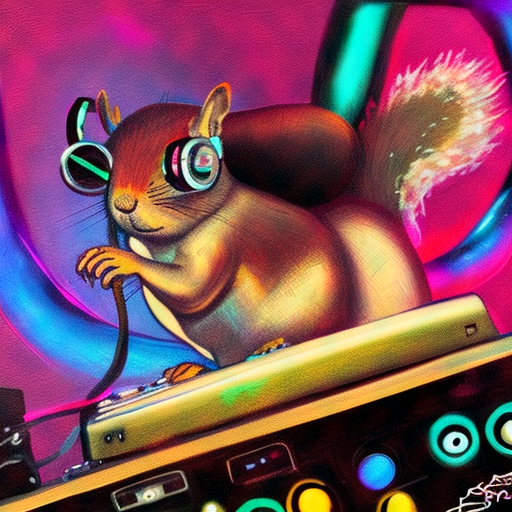
\includegraphics[width=0.62\linewidth]{dwtdct_alpha0_5.PNG}
%         \caption{DWT-DCT Watermark}
%     \end{subfigure}

%     \caption{Visual comparison of different watermarking methods.}
%     \label{fig:watermark_comparison}
% \end{figure*}

\begin{figure*}[t]
    \centering

    % ---------- Row 1: Clean ----------
    \begin{subfigure}[t]{0.19\textwidth}
        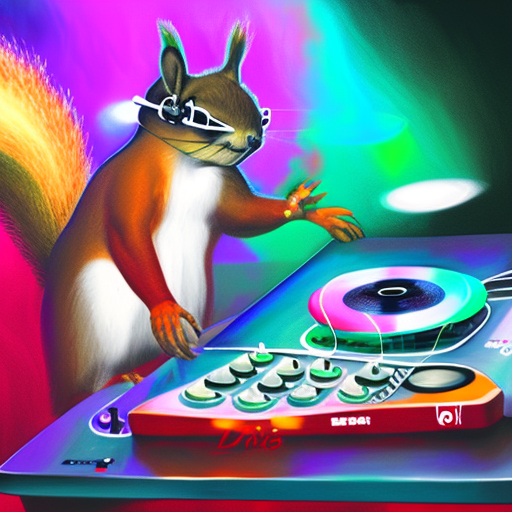
\includegraphics[width=\linewidth]{figures/paper_grid/clean/0000.png}
    \end{subfigure}
    \begin{subfigure}[t]{0.19\textwidth}
        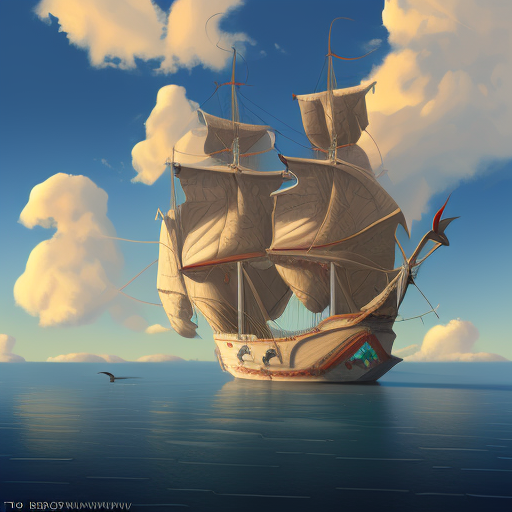
\includegraphics[width=\linewidth]{figures/paper_grid/clean/0002.png}
    \end{subfigure}
    \begin{subfigure}[t]{0.19\textwidth}
        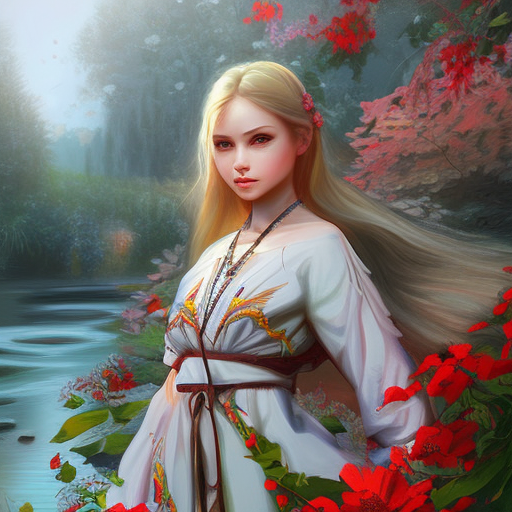
\includegraphics[width=\linewidth]{figures/paper_grid/clean/0004.png}
    \end{subfigure}
    \begin{subfigure}[t]{0.19\textwidth}
        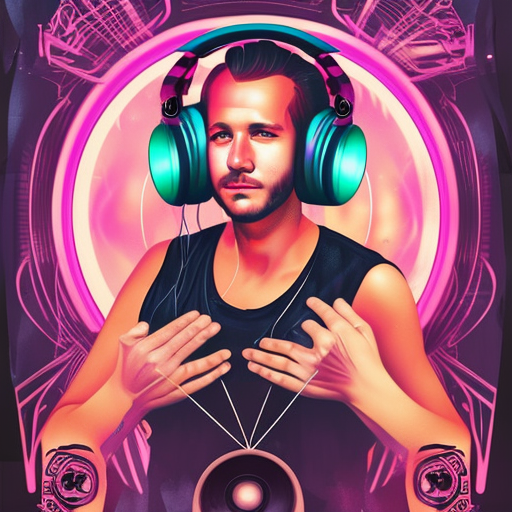
\includegraphics[width=\linewidth]{figures/paper_grid/clean/0016.png}
    \end{subfigure}
    \begin{subfigure}[t]{0.19\textwidth}
        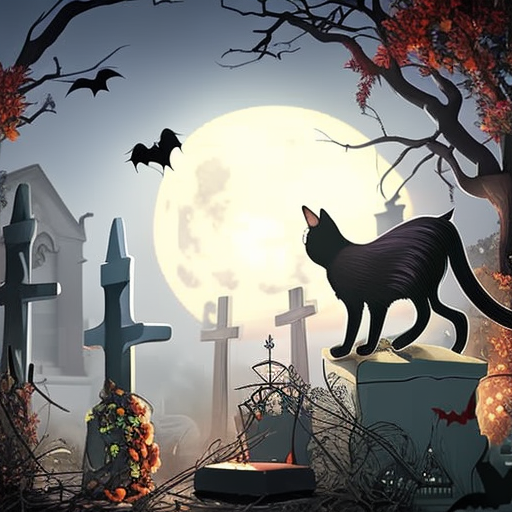
\includegraphics[width=\linewidth]{figures/paper_grid/clean/0021.png}
    \end{subfigure}

    \vspace{2mm}

    % ---------- Row 4: Our ----------
    \begin{subfigure}[t]{0.19\textwidth}
        
\includegraphics[width=\linewidth]{figures/paper_grid/our/0000.png}
    \end{subfigure}
    \begin{subfigure}[t]{0.19\textwidth}
        
\includegraphics[width=\linewidth]{figures/paper_grid/our/0002.png}
    \end{subfigure}
    \begin{subfigure}[t]{0.19\textwidth}
        
\includegraphics[width=\linewidth]{figures/paper_grid/our/0004.png}
    \end{subfigure}
    \begin{subfigure}[t]{0.19\textwidth}
        
\includegraphics[width=\linewidth]{figures/paper_grid/our/0016.png}
    \end{subfigure}
    \begin{subfigure}[t]{0.19\textwidth}
        
\includegraphics[width=\linewidth]{figures/paper_grid/our/0021.png}
    \end{subfigure}

    \vspace{2mm}

    % ---------- Row 5: Tree-Ring ----------
    \begin{subfigure}[t]{0.19\textwidth}
        
\includegraphics[width=\linewidth]{figures/paper_grid/tree-ring/0000.png}
    \end{subfigure}
    \begin{subfigure}[t]{0.19\textwidth}
        
\includegraphics[width=\linewidth]{figures/paper_grid/tree-ring/0002.png}
    \end{subfigure}
    \begin{subfigure}[t]{0.19\textwidth}
        
\includegraphics[width=\linewidth]{figures/paper_grid/tree-ring/0004.png}
    \end{subfigure}
    \begin{subfigure}[t]{0.19\textwidth}
        
\includegraphics[width=\linewidth]{figures/paper_grid/tree-ring/0016.png}
    \end{subfigure}
    \begin{subfigure}[t]{0.19\textwidth}
        
\includegraphics[width=\linewidth]{figures/paper_grid/tree-ring/0021.png}
    \end{subfigure}

    % ---------- Row 2: DFT ----------
    \begin{subfigure}[t]{0.19\textwidth}
        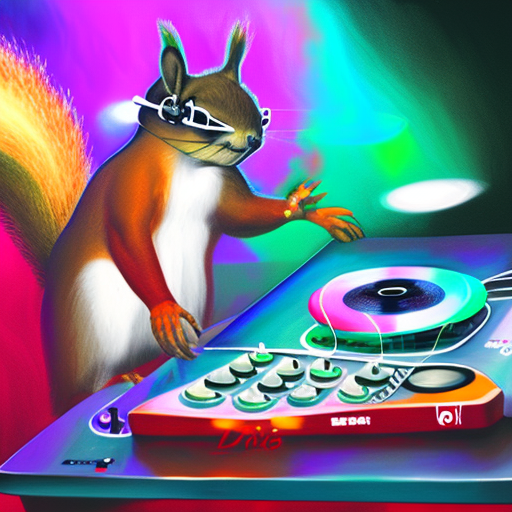
\includegraphics[width=\linewidth]{figures/paper_grid/dft/0000_wm.png}
    \end{subfigure}
    \begin{subfigure}[t]{0.19\textwidth}
        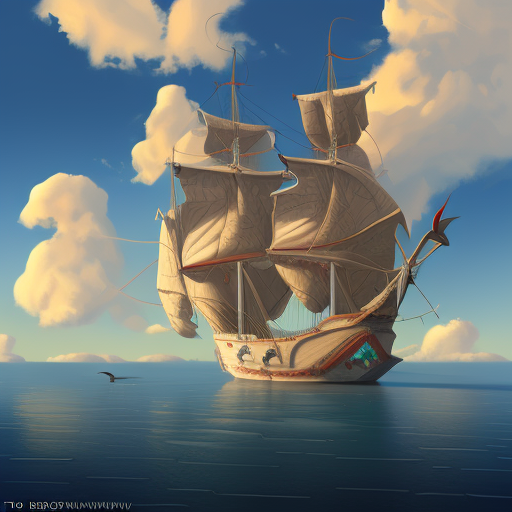
\includegraphics[width=\linewidth]{figures/paper_grid/dft/0002_wm.png}
    \end{subfigure}
    \begin{subfigure}[t]{0.19\textwidth}
        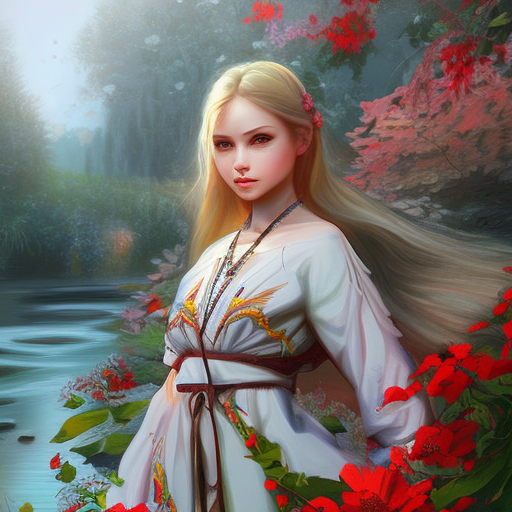
\includegraphics[width=\linewidth]{figures/paper_grid/dft/0004_wm.png}
    \end{subfigure}
    \begin{subfigure}[t]{0.19\textwidth}
        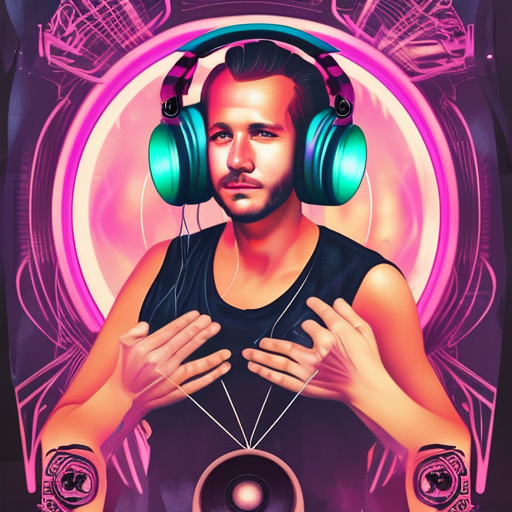
\includegraphics[width=\linewidth]{figures/paper_grid/dft/0016_wm.png}
    \end{subfigure}
    \begin{subfigure}[t]{0.19\textwidth}
        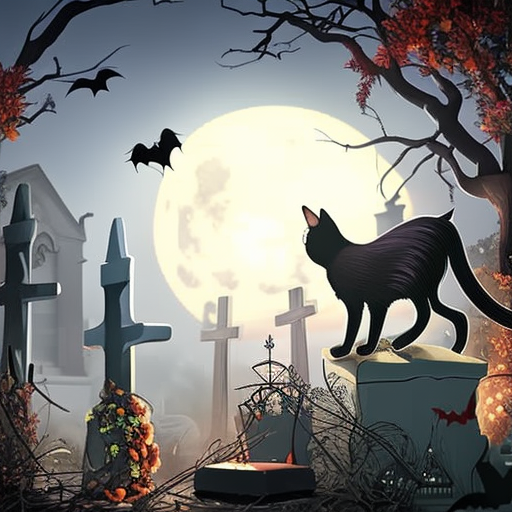
\includegraphics[width=\linewidth]{figures/paper_grid/dft/0021_wm.png}
    \end{subfigure}

    \vspace{2mm}

    % ---------- Row 3: DWT ----------
    \begin{subfigure}[t]{0.19\textwidth}
        
\includegraphics[width=\linewidth]{figures/paper_grid/dwt/0000_wm.png}
    \end{subfigure}
    \begin{subfigure}[t]{0.19\textwidth}
        
\includegraphics[width=\linewidth]{figures/paper_grid/dwt/0002_wm.png}
    \end{subfigure}
    \begin{subfigure}[t]{0.19\textwidth}
        
\includegraphics[width=\linewidth]{figures/paper_grid/dwt/0004_wm.png}
    \end{subfigure}
    \begin{subfigure}[t]{0.19\textwidth}
        
\includegraphics[width=\linewidth]{figures/paper_grid/dwt/0016_wm.png}
    \end{subfigure}
    \begin{subfigure}[t]{0.19\textwidth}
        
\includegraphics[width=\linewidth]{figures/paper_grid/dwt/0021_wm.png}
    \end{subfigure}

    \vspace{2mm}
    \caption{
    Visual comparison across watermarking methods.
    Rows correspond to Clean, Our method, Tree-Ring, DFT and DWT.
    Columns show different image instances.
    }
    \label{fig:watermark_grid}
\end{figure*}


\paragraph{Robustness Evaluation.}
SpiderMark is evaluated under a comprehensive set of post-processing transformations that simulate real-world image distortions. 
Each perturbation is applied to generated images before verification, and both the SpiderMark detector and PSNR baseline (threshold = -4) are evaluated over five independent runs to obtain averaged values. 
The following perturbations are considered:
\begin{itemize}
    \item \textit{Clean}: unmodified images as a reference.
    \item \textit{JPEG-Strong}: aggressive JPEG compression at low quality.
    \item \textit{MsgApp-Combo}: chained resampling and recompression to emulate messaging app transmission.
    \item \textit{Down-Up}: downsampling followed by upsampling to simulate resolution scaling.
    \item \textit{Blur}: Gaussian blur representing optical or motion blur.
    \item \textit{Random Crop}: random resized crops reflecting framing changes.
    \item \textit{Occlusion}: partial masking to assess redundancy and spatial resilience.
    \item \textit{Geom-Warp}: geometric warping and affine distortion.
    \item \textit{Aug-Mix}: composite augmentations used to test generalisation.
\end{itemize}
Evaluation metrics include accuracy and AUROC, averaged across all trials.

\subsection{Quantitative Evaluation}

\begin{table*}[h]
\centering
\caption{Watermark verification performance under various image transformations.
The learned detector (with or without the pattern and mask, PM) is compared against classical
Tree-Ring verification methods \citep{wen2023treeringwatermarksfingerprintsdiffusion}, along with the DFT-Single and DWT-DCT frequency
watermarking baselines. Bold values indicate row-wise best performance. As discussed in
Section~\ref{subsec:auc_limitations}, accuracy at a fixed threshold provides a more reliable
measure of robustness than AUC, since AUC can remain high even when the optimal threshold
varies significantly across different distortions.}
\label{tab:robustness_results_all}
\resizebox{\textwidth}{!}{
\begin{tabular}{lcccccccccc}
\toprule
\multirow{2}{*}{\textbf{Attack}} &
\multicolumn{2}{c}{\textbf{Ours (+PL)}} &
\multicolumn{2}{c}{\textbf{Ours (-PL)}} &
\multicolumn{2}{c}{\textbf{Tree-Ring}} &
\multicolumn{2}{c}{\textbf{DFT-Single}} &
\multicolumn{2}{c}{\textbf{DWT--DCT}} \\
\cmidrule(lr){2-3}
\cmidrule(lr){4-5}
\cmidrule(lr){6-7}
\cmidrule(lr){8-9}
\cmidrule(lr){10-11}
& Acc & AUROC
& Acc & AUROC
& Acc & AUROC
& Acc & AUROC
& Acc & AUROC \\
\midrule

clean           
& \underline{0.9467} & \underline{0.9904}
& 0.8533 & 0.9848
& \textbf{0.9759} & \textbf{0.9971}  
& 0.9090 & 0.9603
& 0.6760 & 0.7199
\\

jpeg\_strong    
& \textbf{0.8720} & \textbf{0.9410}
& \underline{0.7253} & 0.8164
& 0.6627 & \underline{}{0.8772}
& 0.5717 & 0.5730
& 0.6737 & 0.7156
\\

msg\_app\_combo 
& \textbf{0.6813} & \textbf{0.8468}
& 0.5733 & 0.6527
& 0.4747 & \underline{0.8136}
& 0.5223 & 0.5044
& \underline{0.6700} & 0.7113
\\

down\_up        
& \textbf{0.9133} & \textbf{0.9713}
& \underline{0.7600} & 0.8461
& 0.6988 & \underline{0.9576}
& 0.5270 & 0.5164
& 0.6720 & 0.7159
\\

blur            
& \textbf{0.8160} & \textbf{0.8757}
& 0.6427 & 0.6896
& 0.4771 & \underline{0.7777}
& 0.5620 & 0.5717
& \underline{0.6690} & 0.7103
\\

random\_crop    
& \textbf{0.8787} & \underline{0.9503}
& \underline{0.8373} & 0.9102
& 0.7807 & \textbf{0.9565}
& 0.5133 & 0.4912
& 0.5220 & 0.5046
\\

occlusion       
& \textbf{0.9574} & \underline{0.9878}
& 0.9067 & 0.9721
& \underline{0.9325} & \textbf{0.9915}
& 0.9080 & 0.9582
& 0.6603 & 0.6939
\\

geom\_warp      
& \textbf{0.8560} & \underline{0.9381}
& \underline{0.7893} & 0.8734
& 0.7711 & \textbf{0.9412}
& 0.5190 & 0.4909
& 0.5193 & 0.5083
\\

train\_aug\_mix 
& \underline{0.7280} & \underline{0.8620}
& \textbf{0.7400} & 0.8242 
& 0.6337 & \textbf{0.8634}
& 0.5417 & 0.5340
& 0.5360 & 0.5283
\\

\bottomrule
\end{tabular}

}
\end{table*}





\begin{table}[h!]
\centering
\begin{tabular}{lcc}
\hline
\textbf{Attack} & \textbf{Best L1 Thr} & \textbf{Best PSNR Thr} \\
\hline
clean          & -78.2500  & 5.3937 \\
jpeg\_strong   & -82.2500  & 4.9414 \\
msg\_app\_combo & -87.3750  & 4.3452 \\
down\_up       & -82.5625  & 4.6217 \\
blur           & -83.8750  & 4.0488 \\
random\_crop   & -82.6875  & 5.0281 \\
occlusion      & -79.9375  & 5.2857 \\
geom\_warp     & -81.0625  & 5.2801 \\
train\_aug\_mix & -82.1875 & 4.9464 \\
\hline
\end{tabular}
\caption{Optimal thresholds for L1 and PSNR detectors under different attacks. Large threshold shifts indicate that AUC alone is unreliable for evaluating watermark detection robustness.}
\label{tab:threshold_shift}
\end{table}


Across all attack scenarios, SpiderMark achieves significantly higher accuracy and AUROC than the PSNR baseline.  
While PSNR quickly loses discriminative power under pixel-level corruptions, the learned detector maintains reliable separability (AUROC \(>\) 0.7–0.9) even under strong distortions such as compression, blur, or warping.  
Both detectors perform comparably on clean images, confirming that SpiderMark does not compromise the fidelity of unperturbed outputs.

\subsection{Evaluation on COCO Dataset}

To evaluate cross-dataset generalisation, we further assess watermark verification performance on the COCO dataset, which is not used during verifier training. In contrast to prior experiments where the verifier is trained and evaluated on images generated from the Stable Diffusion prompt dataset, this setting tests whether the learned verifier overfits to prompt distributions or generation characteristics seen during training.

Table~\ref{tab:coco_four_methods} reports verification performance under a range of common signal-processing and geometric distortions. Despite being trained solely on Stable Diffusion prompts, our method (SpiderMark) consistently achieves the highest accuracy and AUROC across nearly all attack types on COCO. This includes challenging transformations such as strong JPEG compression, random cropping, geometric warping, and mixed training-time augmentations.

Notably, the performance gap between SpiderMark and prior methods remains substantial even under severe distortions. Tree-Ring shows moderate degradation when transferring to COCO, while frequency-based baselines such as DFT-Single and DWT--DCT exhibit significant performance drops, particularly under geometric and mixed attacks. These results indicate that our verifier does not rely on dataset-specific artifacts, but instead learns watermark-consistent frequency-domain cues that generalise across datasets.

Importantly, this generalisation is achieved without retraining or fine-tuning the verifier on COCO, highlighting the robustness of the proposed verification strategy under distribution shift. Furthermore, FID scores reported in the last row indicate that SpiderMark maintains comparable image quality to other watermarking methods, suggesting that improved robustness does not come at the cost of perceptual degradation.

Overall, these results demonstrate that the proposed watermarking and verification framework generalises effectively to unseen datasets, reinforcing its practicality for real-world deployment where training and test distributions may differ substantially.


\begin{table*}[h]
\centering
\caption{Watermark verification performance on COCO (unseen dataset) under various image transformations.
FID scores are shown as a separate row for each watermarking method.}
\label{tab:coco_four_methods}

\resizebox{.8\textwidth}{!}{
\begin{tabular}{lcccccccc}
\toprule
\multirow{2}{*}{\textbf{Attack / Metric}} &

\multicolumn{2}{c}{\textbf{SpiderMark}} &
\multicolumn{2}{c}{\textbf{Tree-Ring}} &
\multicolumn{2}{c}{\textbf{DFT-Single}} &
\multicolumn{2}{c}{\textbf{DWT--DCT}} \\

\cmidrule(lr){2-3}
\cmidrule(lr){4-5}
\cmidrule(lr){6-7}
\cmidrule(lr){8-9}

& Acc & AUROC
& Acc & AUROC
& Acc & AUROC
& Acc & AUROC \\
\midrule

clean           
& \textbf{0.9733} & \textbf{0.9925}
& 0.8800 & 0.9483
& 0.8840 & 0.9433
& 0.6630 & 0.7062
\\

jpeg\_strong    
& \textbf{0.9000} & \textbf{0.9735}
& 0.7987 & 0.8800
& 0.5793 & 0.5934
& 0.6590 & 0.7009
\\

msg\_app\_combo 
& \textbf{0.7733} & \textbf{0.8820}
& 0.6360 & 0.7556
& 0.5240 & 0.5106
& 0.6567 & 0.6972
\\

down\_up        
& \textbf{0.9133} & \textbf{0.9720}
& 0.7800 & 0.8992
& 0.5130 & 0.4996
& 0.6600 & 0.7026
\\

blur            
& \textbf{0.8173} & \textbf{0.8877}
& 0.6440 & 0.7694
& 0.5540 & 0.5469
& 0.6557 & 0.6975
\\

random\_crop    
& \textbf{0.8240} & \textbf{0.9169}
& 0.7413 & 0.8451
& 0.5177 & 0.4973
& 0.5180 & 0.5011
\\

occlusion       
& \textbf{0.9720} & \textbf{0.9908}
& 0.8560 & 0.9398
& 0.8820 & 0.9402
& 0.6417 & 0.6832
\\

geom\_warp      
& \textbf{0.8373} & \textbf{0.9300}
& 0.7613 & 0.8377
& 0.5147 & 0.4871
& 0.5317 & 0.5173
\\

train\_aug\_mix 
& \textbf{0.7227} & \textbf{0.8389}
& 0.6813 & 0.7730
& 0.5360 & 0.5330
& 0.5360 & 0.5325
\\

\midrule\midrule
FID score  (non-watermarked = 81.743)
& \multicolumn{2}{c}{\underline{83.2103}}
& \multicolumn{2}{c}{83.5059}
& \multicolumn{2}{c}{\textbf{81.7612}}
& \multicolumn{2}{c}{83.3128} \\
\bottomrule

\end{tabular}
}
\end{table*}





\subsection{Semantic Preservation Evaluation using CLIP}

\begin{table}[t]
\centering
\caption{CLIP image--text semantic similarity comparison between clean (unwatermarked) images and different watermarking methods. Higher values indicate better semantic alignment.}
\label{tab:clip_similarity}
\begin{tabular}{lcc}
\toprule
\textbf{Method} & \textbf{COCO} & \textbf{Stable Diffusion} \\
\midrule
Unwatermarked & \textbf{0.3302} & \textbf{0.3615} \\
Tree-Ring             & 0.3296          & 0.3614          \\
Ours (Spidermark)        & 0.3273          & 0.3599          \\
\bottomrule
\end{tabular}
\end{table}


To assess whether watermark injection alters the semantic content of generated images, we evaluate image--text semantic similarity using CLIP. For each image, we compute the cosine similarity between the CLIP image embedding and its corresponding generation prompt. We report the mean CLIP similarity over all samples, with higher values indicating better semantic alignment.

Table~\ref{tab:clip_similarity} presents results on both the COCO and Stable Diffusion verification datasets. Clean (unwatermarked) images achieve mean CLIP similarities of 0.3302 and 0.3615 on COCO and Stable Diffusion, respectively. Tree-Ring produces nearly identical scores, indicating minimal semantic distortion. Our method (OctoWeb) achieves CLIP similarities of 0.3273 on COCO and 0.3599 on Stable Diffusion.

Notably, the semantic gap between our method and clean images is extremely small (no more than 0.003 across both datasets), which is well below commonly accepted thresholds for significant semantic degradation. This demonstrates that the proposed watermarking strategy preserves the semantic alignment between images and their prompts while remaining comparable to state-of-the-art frequency-domain watermarking methods.

Overall, these results confirm that the proposed approach introduces negligible semantic distortion, maintaining high fidelity to the original prompt semantics across different datasets.


\subsection{Ablation — Without Watermark Pattern and Mask for Verification Model}

To evaluate the contribution of the watermark pattern and mask as auxiliary inputs to the verification model, 
we conducted an ablation experiment by removing both components during inference and retraining the model 
under identical conditions. The goal of this analysis is to determine whether the inclusion of watermark-related inputs provides measurable robustness improvements under various image transformations.

Table~\ref{tab:robustness_results_all} compares the performance between the +PL model (with PSNR \& L1), its ablated counterpart,-PL (without PSNR \& L1). 
Across most transformation types, the model +PL achieves higher or comparable accuracy 
and AUROC, particularly under \textit{clean}, \textit{down\_up}, and \textit{occlusion} conditions. The improvements are most pronounced in scenarios where structural or frequency-domain cues from the watermark pattern enhance detection stability against geometric and photometric distortions.

In contrast, the model without the watermark and mask shows slightly lower robustness to severe degradations such as \textit{jpeg\_strong} and \textit{blur}, suggesting that these auxiliary inputs help preserve feature consistency under compression and noise. Nevertheless, both versions maintain a significant advantage over the PSNR baseline, confirming the effectiveness of the learned detector architecture. 
Overall, this ablation study demonstrates that the watermark pattern and mask provide complementary cues that improve verification reliability under challenging transformations.
